\documentclass[12pt,a4paper]{article}
\usepackage[utf8]{inputenc}
\usepackage[spanish,es-tabla]{babel}
\usepackage{geometry}
\usepackage{graphicx}
\usepackage{multirow}
\usepackage{tabularx}
\usepackage{mathptmx}
\usepackage{fancyhdr}
\usepackage{array}
\usepackage[table]{xcolor}
\usepackage{titlesec}
\usepackage{setspace}
\usepackage{microtype}
\usepackage{lastpage}
\usepackage{booktabs}
\usepackage{enumitem}
\usepackage{amsmath}
\usepackage{amsfonts}
\usepackage{amssymb}

\graphicspath{{images/}{../images/}{./}}

\geometry{
    top=4.7cm,
    bottom=2.5cm,
    left=2.5cm,
    right=2.5cm,
    headheight=3.9cm,
    headsep=0.4cm
}

\setstretch{1.15}
\setlength{\parindent}{0pt}
\setlength{\parskip}{0.45em}
\setlength{\tabcolsep}{4pt}

\titleformat{\section}
  {\normalfont\fontsize{12}{14.5}\bfseries}{\thesection.}{0.6em}{\uppercase}
\titlespacing*{\section}
  {0pt}{1.8ex plus 0.4ex minus 0.2ex}{0.6ex plus 0.2ex}

\titleformat{\subsection}
  {\normalfont\fontsize{11.5}{13.5}\bfseries}{\thesubsection.}{0.5em}{}
\titlespacing*{\subsection}
  {0pt}{1.4ex plus 0.3ex minus 0.1ex}{0.4ex plus 0.1ex}

\titleformat{\subsubsection}
  {\normalfont\fontsize{10.5}{12.5}\bfseries\itshape}{\thesubsubsection.}{0.4em}{}
\titlespacing*{\subsubsection}
  {0pt}{1.1ex plus 0.2ex minus 0.1ex}{0.3ex plus 0.1ex}

\newcolumntype{Y}{>{\centering\arraybackslash}X}
\newcolumntype{L}{>{\raggedright\arraybackslash}X}
\newcolumntype{C}{>{\centering\arraybackslash}X}

\definecolor{headerblue}{RGB}{26, 54, 93}
\definecolor{darkblue}{RGB}{43, 108, 176}
\definecolor{lightgraybg}{RGB}{248, 248, 248}
\definecolor{tableheader}{RGB}{232, 238, 246}

\newcommand{\docCodigo}{TI-SIGE-ENT-F3-002}
\newcommand{\docVersion}{1.0}
\newcommand{\docProceso}{DESARROLLO CORE / CATÁLOGOS MAESTROS}
\newcommand{\docElaboracion}{14/09/2026}
\newcommand{\docRevision}{14/09/2026}
\newcommand{\docTitulo}{DATOS INICIALES Y CATÁLOGOS INSTITUCIONALES}
\newcommand{\docOrganizacion}{FACULTAD DE INGENIERÍA EN SISTEMAS, ELECTRÓNICA E INDUSTRIAL}
\newcommand{\docSubOrganizacion}{CARRERA DE INGENIERÍA DE SOFTWARE}

\newcommand{\encabezadofrecuente}{%
    \renewcommand{\arraystretch}{1.15}%
    \noindent\makebox[\textwidth][c]{%
    \begin{tabularx}{\textwidth}{|>{\centering\arraybackslash}m{2.8cm}|Y|>{\centering\arraybackslash}m{4.8cm}|}
        \hline
        \multirow{4}{2.8cm}{\centering\raisebox{-1.15cm}{
\includegraphics[width=2.5cm,height=2.0cm,keepaspectratio]{images/logo.png}}}
        & \textbf{\fontsize{9}{11}\selectfont \docOrganizacion} 
        & \textbf{\fontsize{8}{10}\selectfont CÓDIGO:} \fontsize{8}{10}\selectfont \docCodigo \\
        \cline{3-3}
        & \textbf{\fontsize{8.5}{10.5}\selectfont \docSubOrganizacion} 
        & \textbf{\fontsize{8}{10}\selectfont VERSIÓN:} \fontsize{8}{10}\selectfont \docVersion \\
        \cline{2-3}
        & \textbf{\fontsize{8}{10}\selectfont PROCESO:} \fontsize{8}{10}\selectfont \docProceso 
        & \textbf{\fontsize{8}{10}\selectfont ELABORACIÓN:} \fontsize{8}{10}\selectfont \docElaboracion \\
        \cline{2-3}
        & \textbf{\fontsize{8.5}{10.5}\selectfont \docTitulo} 
        & \textbf{\fontsize{8}{10}\selectfont ÚLTIMA REVISIÓN:} \fontsize{8}{10}\selectfont \docRevision \\
        \hline
    \end{tabularx}%
    }%
}

\pagestyle{fancy}
\fancyhf{}
\fancyhead[C]{\encabezadofrecuente}
\fancyfoot[C]{\fontsize{10}{12}\selectfont Página \thepage\ de \pageref{LastPage}}
\renewcommand{\headrulewidth}{0pt}

\begin{document}

\noindent{\fontsize{10.5}{12.5}\selectfont \textbf{Integrantes:} Heidi Villavicencio \quad$\vert$\quad Steeven Toala \quad$\vert$\quad Nixon Hurtado \quad$\vert$\quad Andrea Vásquez}

\vspace{0.25cm}

\section{Título}
\textbf{Denominación del Entregable:} Datos Iniciales y Catálogos Institucionales -- Código EDT: 3.2

\section{Introducción}
Para que el sistema SIGE sea operativo y refleje fielmente la estructura orgánica de la FISEI, se requiere la inicialización de los catálogos maestros y los datos semilla (Seeding). En esta actividad se desarrolló el módulo de inicialización automatizada que precarga en la base de datos relacional las carreras académicas, roles de seguridad institucional, períodos lectivos vigentes y el catálogo estandarizado de tipologías de actividades de docencia, investigación y vinculación.

\section{Objetivo}
\subsection{Objetivo General}
Poblar y parametrizar los catálogos institucionales maestros y datos iniciales en PostgreSQL 18, asegurando la disponibilidad de datos de referencia para el funcionamiento del SGC.
\subsection{Objetivos Específicos}
\begin{itemize}[leftmargin=1.5em, itemsep=2pt]
    \item Poblar las tablas maestras de Roles, Facultades, Carreras y Períodos Académicos.
    \item Estandarizar el catálogo de 28 tipos de actividades académicas según el Manual SGC.
    \item Crear los usuarios institucionales de prueba con roles asignados para validación del ciclo completo.
\end{itemize}

\section{Alcance}
\subsection{Límites del Entregable (In-Scope)}
\begin{itemize}[leftmargin=1.5em, itemsep=2pt]
    \item Script de inicialización \texttt{seed.sql} y módulo automatizado \texttt{init.js}.
    \item Validación de idempotencia: el script puede ejecutarse múltiples veces sin duplicar registros.
\end{itemize}
\subsection{Exclusiones (Out-of-Scope)}
\begin{itemize}[leftmargin=1.5em, itemsep=2pt]
    \item Migración masiva de expedientes de semestres anteriores a 2026.
\end{itemize}

\section{Definiciones}
\begin{itemize}[leftmargin=1.5em, itemsep=2pt]
    \item \textbf{Database Seeding:} Proceso de poblar inicialmente una base de datos con un conjunto predeterminado de datos maestros.
    \item \textbf{Idempotencia:} Propiedad de una operación que puede ser ejecutada varias veces produciendo el mismo resultado que tras la primera ejecución.
    \item \textbf{Catálogo SGC:} Clasificador institucional de actividades docentes que rige las horas asignadas en los planes de trabajo.
\end{itemize}

\section{Responsabilidades}
\begin{itemize}[leftmargin=1.5em, itemsep=2pt]
    \item \textbf{Nixon Hurtado (Responsable EDT 3.2):} Desarrollo del script de semillado y verificación de catálogos.
    \item \textbf{Heidi Villavicencio (Analista):} Validación de la concordancia de los códigos de actividad con el formato P7-T1.
    \item \textbf{Ing. Paulo Torres (Docente Evaluador):} Aprobación de los datos iniciales y catálogos institucionales.
\end{itemize}

\section{Normativa Legal y Técnica}
\begin{itemize}[leftmargin=1.5em, itemsep=2pt]
    \item \textbf{Manual de Calidad SGC - FISEI UTA:} Catálogo de Actividades y Funciones Docentes.
\end{itemize}

\section{Método, Políticas y Contenidos}
Se utilizó un script de inicialización transaccional con sentencias \texttt{ON CONFLICT DO NOTHING}. En la Figura \ref{fig:f3_02_seed} se presenta el esquema de catálogos y usuarios inicializados.

\begin{figure}[htbp]
    \centering
    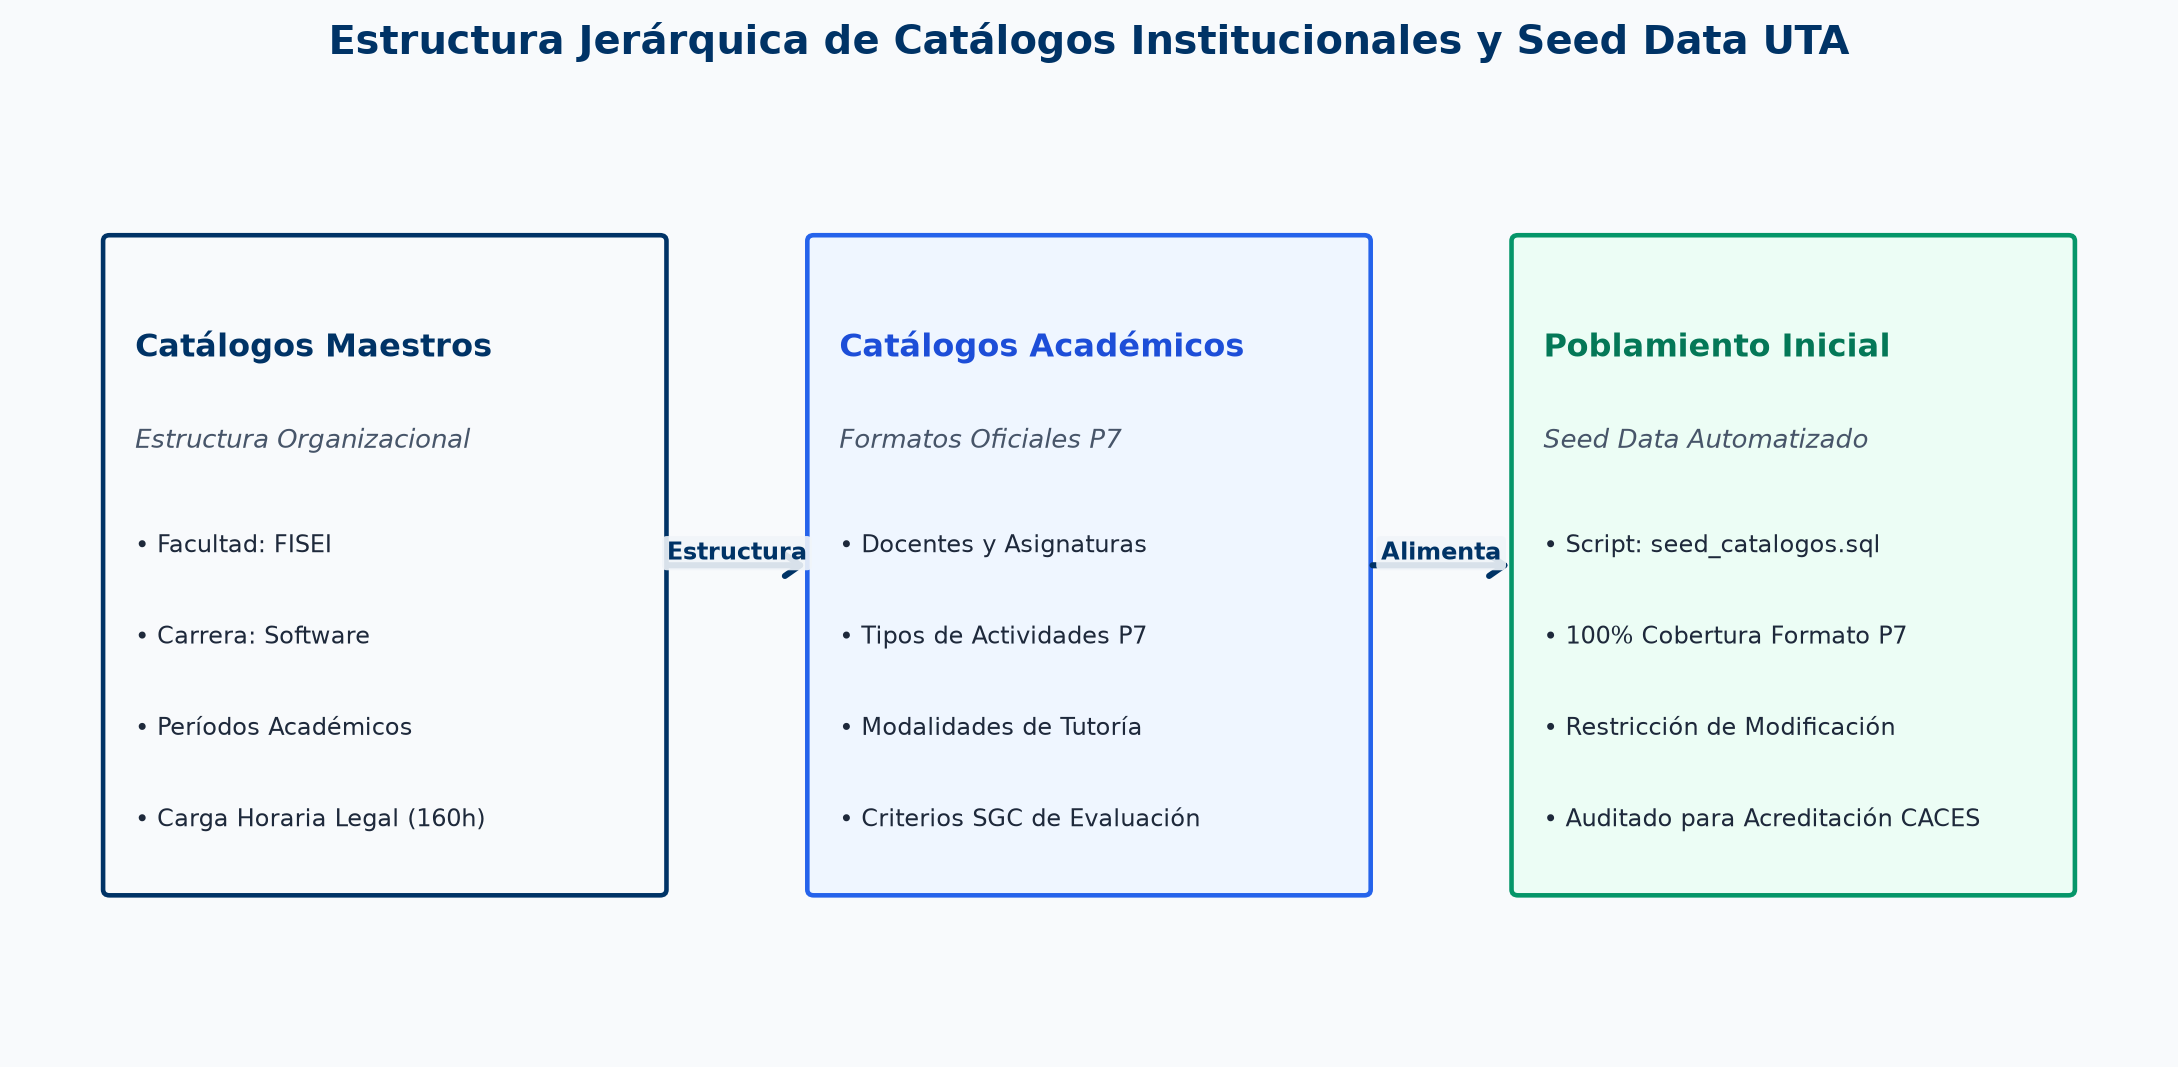
\includegraphics[width=0.88\textwidth,height=5.2cm,keepaspectratio]{images/f3_02_catalogos_institucionales_seed.png}
    \caption{Mapa de Catálogos Institucionales y Semillado Inicial en PostgreSQL 18.}
    \label{fig:f3_02_seed}
\end{figure}

\section{Descripción de actividades}
\subsection{Catálogo Maestro de Actividades Académicas SGC}
\begin{table}[htbp]
\centering
\small
\renewcommand{\arraystretch}{1.2}
\begin{tabularx}{\textwidth}{|c|>{\bfseries}m{3.2cm}|c|X|}
\hline
\rowcolor{tableheader}
\textbf{Código SGC} & \textbf{Categoría} & \textbf{Horas Máx.} & \textbf{Descripción de Actividad Institucional} \\
\hline
\texttt{ACT-DOC-01} & Docencia de Aula & 16 h/sem & Impartición de clases presenciales en asignaturas curriculares. \\
\hline
\texttt{ACT-DOC-02} & Preparación Clases & 8 h/sem & Planificación didáctica, elaboración de material y exámenes. \\
\hline
\texttt{ACT-DOC-03} & Tutorías Académicas & 4 h/sem & Atención extracurricular y refuerzo pedagógico a estudiantes. \\
\hline
\texttt{ACT-INV-01} & Proyecto Investigación & 10 h/sem & Dirección y ejecución de proyectos de investigación aprobados DIS. \\
\hline
\texttt{ACT-INV-02} & Publicación Científica & 6 h/sem & Redacción de artículos científicos en revistas Scopus/Latindex. \\
\hline
\texttt{ACT-VIN-01} & Vinculación Sociedad & 8 h/sem & Ejecución de programas de vinculación comunitaria institucional. \\
\hline
\texttt{ACT-GES-01} & Coordinación / Gestión & 10 h/sem & Desempeño de funciones directivas de área o comisiones de calidad. \\
\hline
\end{tabularx}
\caption{Muestra del Catálogo Estandarizado de Actividades SGC.}
\label{tab:catalogos_seed}
\end{table}

\subsection{Cuentas Institucionales Iniciales}
Se parametrizaron 4 cuentas institucionales representativas con contraseñas cifradas con bcrypt (costo 10) para Docente, Coordinador de Área, Coordinador de Carrera y Administrador General.

\section{Firmas de Responsabilidad}

\noindent
\renewcommand{\arraystretch}{1.2}
\begin{tabularx}{\textwidth}{|>{\raggedright\arraybackslash}m{2.9cm}|>{\raggedright\arraybackslash}X|>{\centering\arraybackslash}m{4.6cm}|>{\centering\arraybackslash}m{2.3cm}|}
    \hline
    \rowcolor{tableheader}
    \textbf{ACCIÓN} & \textbf{NOMBRE Y CARGO} & \textbf{FIRMA} & \textbf{FECHA} \\
    \hline
    \textbf{Elaborado por:} & Heidi Villavicencio\newline Analista de Calidad / UI-UX & \parbox[c]{4.4cm}{\centering\vspace{4pt}
\includegraphics[height=1.5cm,width=4.0cm,keepaspectratio]{images/firma_heidi.png}\vspace{4pt}} & 14/09/2026 \\
    \hline
    \textbf{Revisado por:} & Steeven Toala\newline Líder de Proyecto / Arquitecto & \parbox[c]{4.4cm}{\centering\vspace{4pt}
\includegraphics[height=1.5cm,width=4.0cm,keepaspectratio]{images/firma_steveen.png}\vspace{4pt}} & 14/09/2026 \\
    \hline
    \textbf{Aprobado por:} & Ing. Paulo Torres, Mg.\newline Docente Evaluador -- Gestión Proyectos & \parbox[c]{4.4cm}{\centering\vspace{8pt}\textbf{\textcolor{gray!80}{\scriptsize [ PENDIENTE DE APROBACIÓN ]}}\vspace{8pt}} & \textbf{\textcolor{gray!90}{Pendiente}} \\
    \hline
\end{tabularx}

\vspace{0.4cm}

\section{Control de Cambios}

\noindent
\renewcommand{\arraystretch}{1.2}
\begin{tabularx}{\textwidth}{|>{\hsize=0.45\hsize\centering\arraybackslash}X|>{\hsize=1.55\hsize\raggedright\arraybackslash}X|>{\hsize=1.2\hsize\raggedright\arraybackslash}X|>{\hsize=0.8\hsize\centering\arraybackslash}X|}
    \hline
    \rowcolor{tableheader}
    \textbf{Versión} & \textbf{Descripción del cambio} & \textbf{Responsable del cambio} & \textbf{Fecha de aprobación} \\
    \hline
    1.0 & Emisión inicial del entregable según EDT del Tablero Trello & Equipo de Proyecto SIGE & 14/09/2026 \\
    \hline
\end{tabularx}

\vspace{0.4cm}

\section{Anexos}
\begin{itemize}[leftmargin=1.5em]
\item \textbf{Anexo 1:} Lista Completa de los 28 Tipos de Actividades Académicas Parametrizadas.
\end{itemize}

\end{document}
